\chapter{Elements in the Universe and on Earth}\label{ch:g9:elements-universe-earth}

The calcium in your bones, the iron in your blood and the oxygen you
breathe were not made on Earth. They were made inside stars that lived
and died before the Sun was born, and they have been passed from rock to
sea, from sea to plant, from plant to animal, for billions of years. Some
elements are everywhere, others rare. Which elements make up the stars,
the Earth, the oceans --- and us?

\begin{recall}
A \omterm{def:g9:inside-the-atom:element}{chemical element} is the set of \omterm{def:g7:atoms-and-molecules:atom}{atoms} with the same \omterm{def:g9:inside-the-atom:atomic-number}{atomic number} $Z$;
the mass of an \omterm{def:g7:atoms-and-molecules:atom}{atom} is close to $A \times \qty{1.67e-27}{kg}$, where $A$
is its \omterm{def:g9:inside-the-atom:atomic-number}{mass number} (\cref{ch:g9:inside-the-atom}). The \omterm{def:g9:periodic-table-first-look:periodic-table}{periodic table}
lists the 118 elements by \omterm{def:g9:inside-the-atom:atomic-number}{atomic number}
(\cref{ch:g9:periodic-table-first-look}). \omterm{def:g4:air-a-mixture-of-gases:air}{Air} is about four fifths
nitrogen and one fifth oxygen (\cref{ch:g4:air-a-mixture-of-gases}).
\end{recall}

\section{Elements of the stars}

\begin{definition}[Abundance]\label{def:g9:elements-universe-earth:abundance}
The \emph{abundance}\index{abundance} of an element in a body of matter
--- a star, the Earth's crust, the ocean, a living being --- is its share
of the total mass, usually given in percent.
\end{definition}

\begin{proposition}[The Sun is hydrogen and helium]\label{prop:g9:elements-universe-earth:sun}
% ledger: ab:sun-X, ab:sun-Y, ab:sun-Z
The surface of the Sun is, by mass, about \qty{74}{\percent} hydrogen
and \qty{25}{\percent} helium; all the other elements together make up
only about \qty{1.3}{\percent}. Most of the visible matter of the
Universe has a similar composition: hydrogen and helium, with a pinch of
everything else.
\end{proposition}

\begin{proposition}[Elements made in stars]\label{prop:g9:elements-universe-earth:stars}
Hydrogen and most of the helium were formed in the first minutes of the
Universe. Nearly all the heavier elements --- carbon, oxygen, iron, gold
--- were made later, inside stars, and scattered into space when stars
exploded. New stars and planets formed from that enriched dust. How the
stars do it is told in the physics book.
\end{proposition}

\begin{omfigure}
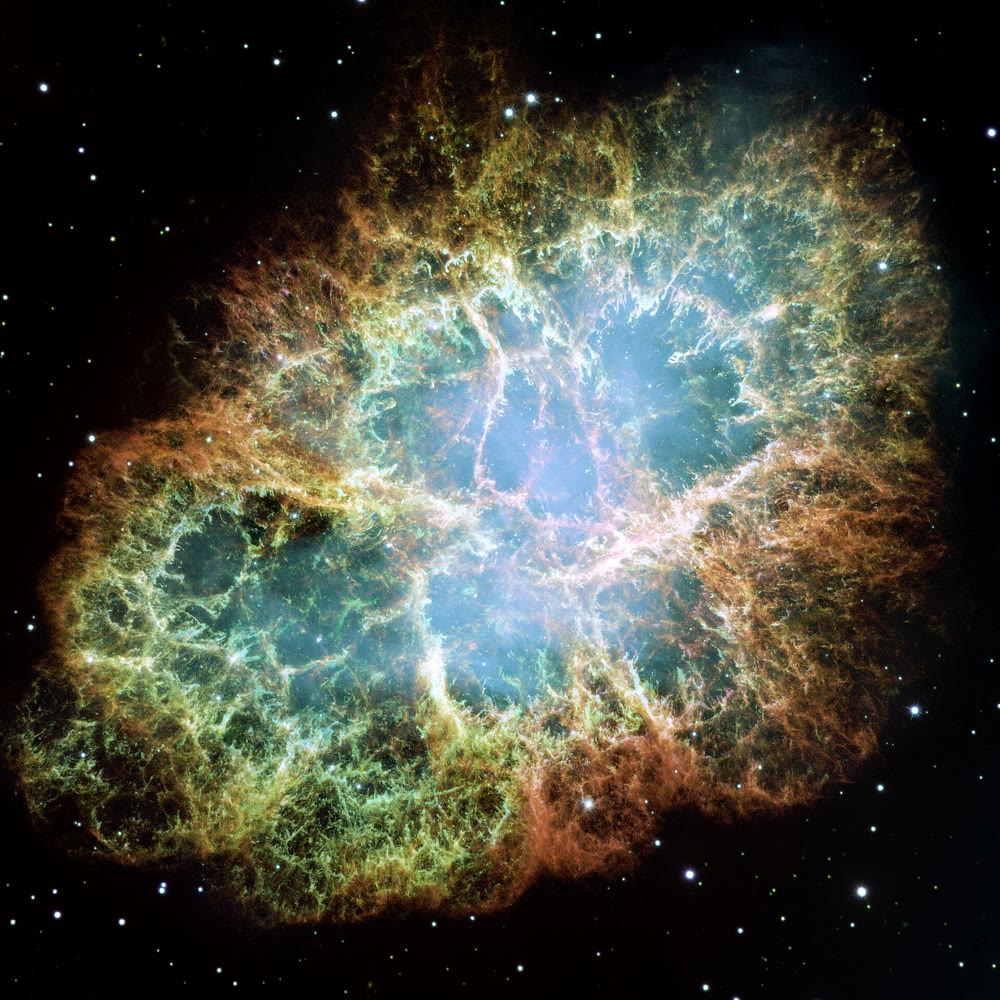
\includegraphics[width=0.45\linewidth]{images/book1/crab-nebula.jpg}

{\small The Crab Nebula, the cloud left by a star that exploded nearly a
thousand years ago, spreading new elements into space (NASA, ESA,
J.~Hester and A.~Loll).}
\end{omfigure}

\section{The Earth}

\begin{proposition}[The Earth's crust]\label{prop:g9:elements-universe-earth:crust}
% ledger: ab:crust-O, ab:crust-Si, ab:crust-Al, ab:crust-Fe, ab:crust-Ca, ab:crust-Na, ab:crust-K, ab:crust-Mg, ab:crust-first10
The thin rocky skin of the Earth, the crust, is almost half oxygen and
more than a quarter silicon by mass: rocks and sand are mostly oxides of
silicon and of a few \omterm{def:g9:periodic-table-first-look:metal}{metals}. Eight elements --- oxygen, silicon,
aluminium, iron, calcium, sodium, potassium, magnesium --- make up about
\qty{99}{\percent} of it. Hydrogen and helium, so common in the stars,
are rare: the light gases escaped from the young Earth.
\end{proposition}

\begin{remark}[Inside the Earth]\label{rem:g9:elements-universe-earth:core}
The crust is not the whole Earth. Iron, heavy, sank towards the centre
when the young Earth was molten: the core of the Earth is mostly iron,
with some nickel.
\end{remark}

\begin{proposition}[The oceans and the air]\label{prop:g9:elements-universe-earth:ocean}
% ledger: sea:salts-share, sea:NaCl-ions, sea:MgSO4-ions, air:N2, air:O2
Sea water is mostly water --- hydrogen and oxygen --- with about
\qty{3.5}{\percent} of dissolved salts by mass. Among the dissolved \omterm{def:g9:ions:ion}{ions},
chloride and sodium make up about \qty{85}{\percent}, magnesium and
sulfate another \qty{10}{\percent}. The \omterm{def:g4:air-a-mixture-of-gases:air}{air} is mostly nitrogen and
oxygen.
\end{proposition}

\begin{omfigure}
\begin{tikzpicture}
\begin{axis}[xbar, width=0.40\linewidth, height=5.4cm, xmin=0, xmax=85,
    bar width=7pt, symbolic y coords={Mg,K,Na,Ca,Fe,Al,Si,O}, ytick=data,
    xlabel={percent of the mass}, title={\small the Earth's crust},
    nodes near coords, nodes near coords style={font=\scriptsize},
    tick label style={font=\small}, label style={font=\small},
    axis lines*=left, enlarge y limits=0.08]
% ledger: ab:crust-O, ab:crust-Si, ab:crust-Al, ab:crust-Fe, ab:crust-Ca, ab:crust-Na, ab:crust-K, ab:crust-Mg
\addplot[fill=omDef!45, draw=omDef] coordinates {(46.6,O) (27.7,Si) (8.1,Al)
  (5.0,Fe) (3.6,Ca) (2.8,Na) (2.6,K) (2.1,Mg)};
\end{axis}
\end{tikzpicture}\hfill
\begin{tikzpicture}
\begin{axis}[xbar, width=0.40\linewidth, height=5.4cm, xmin=0, xmax=85,
    bar width=7pt, symbolic y coords={{P},{N},{Ca},{H},{C},{O}}, ytick=data,
    xlabel={percent of the mass}, title={\small a human body},
    nodes near coords, nodes near coords style={font=\scriptsize},
    tick label style={font=\small}, label style={font=\small},
    axis lines*=left, enlarge y limits=0.1]
% ledger: body:atoms-O, body:atoms-C, body:atoms-H, body:atoms-N, body:atoms-Ca, body:atoms-P (masses = atoms x atomic mass, over 70 kg)
\addplot[fill=omProp!45, draw=omProp] coordinates {(61.1,O) (22.9,C) (10.1,H)
  (1.3,N) (1.5,Ca) (0.7,P)};
\end{axis}
\end{tikzpicture}

{\small \omterm{def:g9:elements-universe-earth:abundance}{Abundances} by mass. Left: the eight main elements of the Earth's
crust. Right: the six main elements of a lean adult human body
(computed from estimated numbers of \omterm{def:g7:atoms-and-molecules:atom}{atoms}).}
\end{omfigure}

\section{The human body}

\begin{proposition}[What we are made of]\label{prop:g9:elements-universe-earth:body}
% ledger: body:atoms-O, body:atoms-C, body:atoms-H, body:atoms-N, body:atoms-Ca, body:atoms-P, body:atoms-total
By mass, a lean adult body is about \qty{61}{\percent} oxygen,
\qty{23}{\percent} carbon and \qty{10}{\percent} hydrogen --- mostly in
water and in the \omterm{def:g7:atoms-and-molecules:molecule}{molecules} of life --- followed by nitrogen, calcium (in
bones and teeth) and phosphorus. Counted in \omterm{def:g7:atoms-and-molecules:atom}{atoms} rather than in mass,
the order changes: there are more hydrogen \omterm{def:g7:atoms-and-molecules:atom}{atoms} in a body than all
other \omterm{def:g7:atoms-and-molecules:atom}{atoms} together, because hydrogen \omterm{def:g7:atoms-and-molecules:atom}{atoms} are so light. A body of
\qty{70}{kg} holds about $7 \times 10^{27}$ \omterm{def:g7:atoms-and-molecules:atom}{atoms}.
\end{proposition}

\begin{method}[Reading an abundance chart]\label{met:g9:elements-universe-earth:read}
\begin{enumerate}
  \item Check what is measured: mass (most charts) or number of \omterm{def:g7:atoms-and-molecules:atom}{atoms}.
  \item Read the share of each element; add those of the main ones to
        see how much they cover.
  \item To compare two bodies, look for the elements common to both and
        for those found in one only.
\end{enumerate}
Oxygen tops both charts of this chapter: it is the commonest element of
the crust and of the human body by mass.
\end{method}

\section{The same atoms, recycled}

\begin{example}[The journey of a carbon atom]\label{ex:g9:elements-universe-earth:journey}
A carbon \omterm{def:g7:atoms-and-molecules:atom}{atom} made in a star long ago can sit for millions of years in
limestone, be released as carbon dioxide by a volcano, be taken up by a
leaf, become part of a sugar in a fruit, pass into an animal that eats
the fruit, and be breathed out again as carbon dioxide. \omterm{def:g7:atoms-and-molecules:atom}{Atoms} are not
destroyed by \omterm{def:g5:irreversible-changes:chemical-change}{chemical changes}: they are passed on.
\end{example}

\begin{omfigure}
\begin{tikzpicture}[font=\small,
    box/.style={draw=omDef, fill=omDef!6, rounded corners=2pt, align=center,
      minimum height=0.85cm, text width=2.3cm}]
  \node[box] (a) at (0,2.2) {in a rock\\ (limestone)};
  \node[box] (b) at (4.3,2.2) {in the air\\ (\ce{CO2})};
  \node[box] (c) at (8.6,2.2) {in a leaf\\ (sugar)};
  \node[box] (d) at (8.6,0) {in an animal};
  \node[box] (e) at (4.3,0) {breathed out\\ (\ce{CO2})};
  \draw[->, thick, omProp] (a) -- node[above, font=\footnotesize] {volcano} (b);
  \draw[->, thick, omProp] (b) -- (c);
  \draw[->, thick, omProp] (c) -- node[right, font=\footnotesize] {eaten} (d);
  \draw[->, thick, omProp] (d) -- (e);
  \draw[->, thick, omProp] (e) -- (b);
\end{tikzpicture}

{\small A carbon \omterm{def:g7:atoms-and-molecules:atom}{atom} passes from rock to \omterm{def:g4:air-a-mixture-of-gases:air}{air} to leaf to animal and back to
the \omterm{def:g4:air-a-mixture-of-gases:air}{air}: the \omterm{def:g7:atoms-and-molecules:atom}{atom} itself is never destroyed.}
\end{omfigure}

\begin{omfigure}
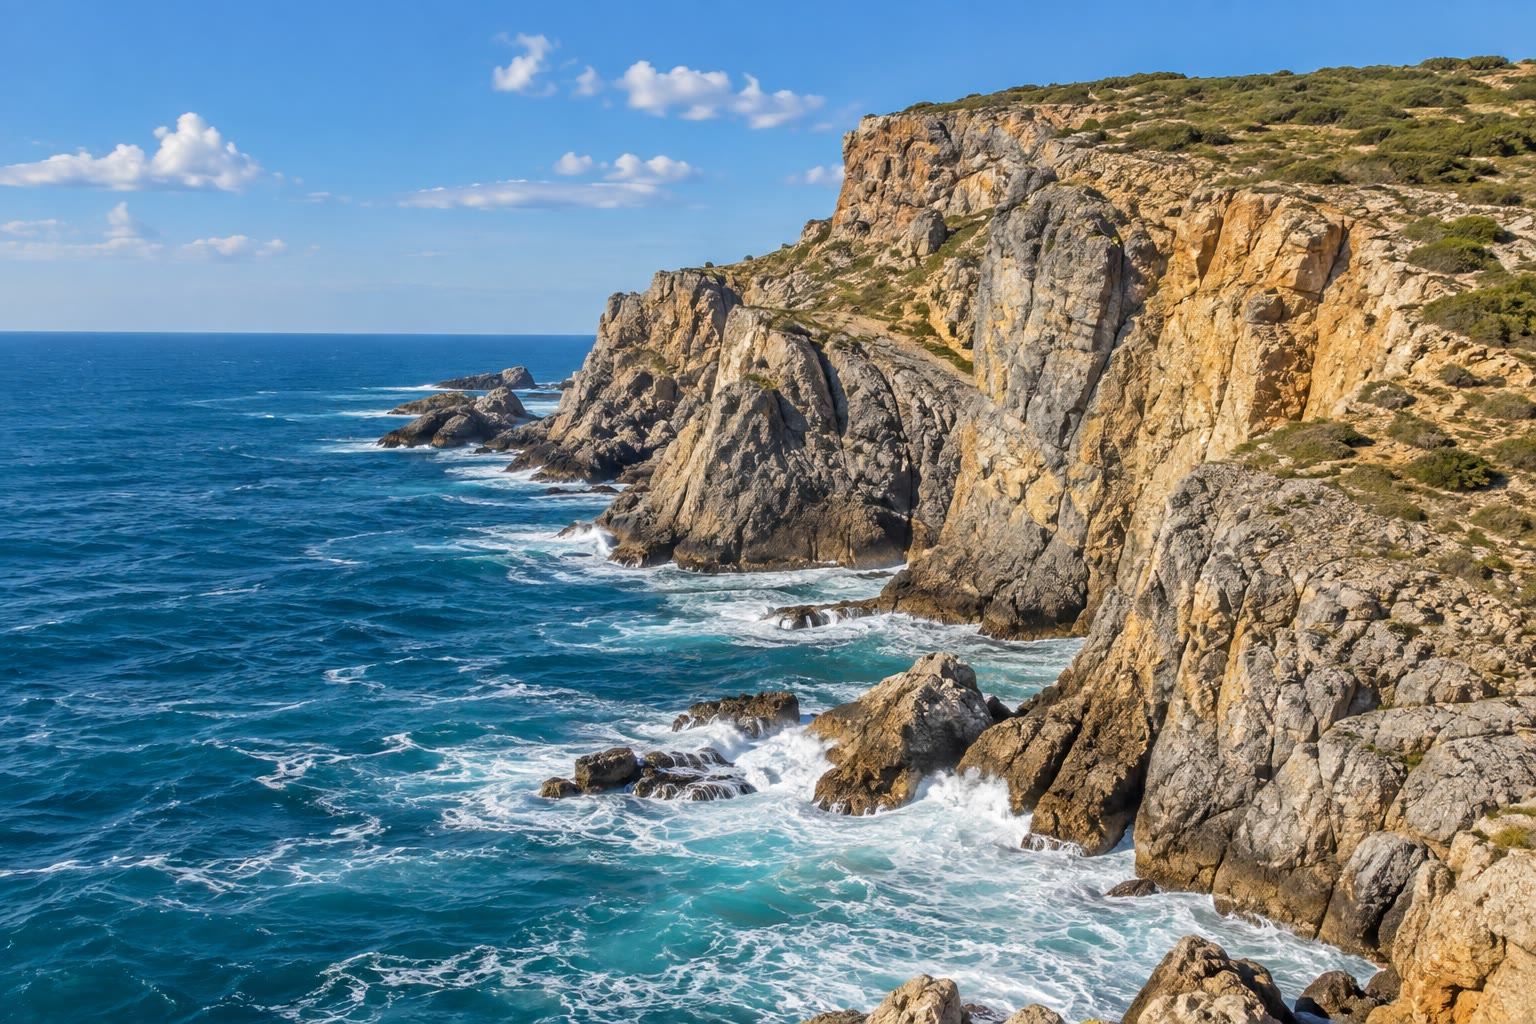
\includegraphics[width=0.55\linewidth]{images/book1/ai/g9-coastal-cliff.jpg}

{\small Rock, sea and \omterm{def:g4:air-a-mixture-of-gases:air}{air}: three very different \omterm{def:g6:pure-substances-and-mixtures:mixture}{mixtures} of the same
elements.}
\end{omfigure}

\section{Exercises}

\begin{exercise}[$\star$]\label{exo:g9:elements-universe-earth:1}
Which two elements make up almost all of the Sun?
\end{exercise}

\begin{exercise}[$\star$]\label{exo:g9:elements-universe-earth:2}
Which element is the most abundant in the Earth's crust? In the human
body (by mass)?
\end{exercise}

\begin{exercise}[$\star$]\label{exo:g9:elements-universe-earth:3}
Where were most of the elements heavier than helium made?
\end{exercise}

\begin{exercise}[$\star$]\label{exo:g9:elements-universe-earth:4}
What percentage of the mass of sea water is dissolved salt?
\end{exercise}

\begin{exercise}[$\star\star$]\label{exo:g9:elements-universe-earth:5}
Using the crust chart, add the shares of oxygen and silicon. What
fraction of the crust is that, roughly?
\end{exercise}

\begin{exercise}[$\star\star$]\label{exo:g9:elements-universe-earth:6}
Why is there so little hydrogen and helium in the Earth's crust, when
the Sun is made almost entirely of them?
\end{exercise}

\begin{exercise}[$\star\star$]\label{exo:g9:elements-universe-earth:7}
What mass of carbon is there in a \qty{70}{kg} body that is
\qty{23}{\percent} carbon?
\end{exercise}

\begin{exercise}[$\star\star$]\label{exo:g9:elements-universe-earth:8}
Why is oxygen the commonest element of the body by mass, while hydrogen is
the commonest by number of \omterm{def:g7:atoms-and-molecules:atom}{atoms}?
\end{exercise}

\begin{exercise}[$\star\star$]\label{exo:g9:elements-universe-earth:9}
A \qty{1000}{kg} block of granite is a typical piece of the crust. Using
the chart, what mass of aluminium does it hold, about?
\end{exercise}

\begin{exercise}[$\star\star$]\label{exo:g9:elements-universe-earth:10}
Which elements appear among the main elements of both the crust and the
human body?
\end{exercise}

\begin{exercise}[$\star\star\star$]\label{exo:g9:elements-universe-earth:11}
A \qty{70}{kg} body holds about \qty{1.06}{kg} of calcium. Compute the
mass of one calcium \omterm{def:g7:atoms-and-molecules:atom}{atom} ($A = 40$), then the number of calcium \omterm{def:g7:atoms-and-molecules:atom}{atoms}.
Write it in scientific notation.
\end{exercise}

\begin{exercise}[$\star\star\star$]\label{exo:g9:elements-universe-earth:12}
The \omterm{def:g7:atoms-and-molecules:atom}{atoms} of your body have all been part of other things before. Use
the journey of a carbon \omterm{def:g7:atoms-and-molecules:atom}{atom} to explain why the total number of carbon
\omterm{def:g7:atoms-and-molecules:atom}{atoms} on Earth hardly changes.
\end{exercise}

\section{Problem: How Many Atoms Am I?}

\begin{problem}[{Weekend problem --- from an abundance chart to the number
of oxygen atoms in a human body}]
\label{pb:g9:elements-universe-earth:1}
% ledger: body:atoms-O, body:atoms-total
A lean adult of \qty{70}{kg} is, by mass, about \qty{61}{\percent}
oxygen, \qty{23}{\percent} carbon and \qty{10}{\percent} hydrogen. Take
the mass of a \omterm{def:g9:inside-the-atom:proton}{nucleon} as \qty{1.67e-27}{kg}; an oxygen \omterm{def:g7:atoms-and-molecules:atom}{atom} has 16
\omterm{def:g9:inside-the-atom:proton}{nucleons}, a carbon \omterm{def:g7:atoms-and-molecules:atom}{atom} 12, a hydrogen \omterm{def:g7:atoms-and-molecules:atom}{atom} 1. \omterm{def:g9:inside-the-atom:nucleus}{Electrons} are neglected.

\medskip
\noindent\textbf{Part I --- The masses.}
\begin{enumerate}
  \item Compute the mass of oxygen in the body.
  \item Compute the mass of carbon and of hydrogen.
  \item What percentage of the mass do these three elements make up
        together?
  \item Most of this oxygen and hydrogen is in one compound. Which?
\end{enumerate}

\medskip
\noindent\textbf{Part II --- One \omterm{def:g7:atoms-and-molecules:atom}{atom}.}
\begin{enumerate}[resume]
  \item Compute the mass of one oxygen \omterm{def:g7:atoms-and-molecules:atom}{atom}.
  \item Compute the mass of one carbon \omterm{def:g7:atoms-and-molecules:atom}{atom} and of one hydrogen \omterm{def:g7:atoms-and-molecules:atom}{atom}.
  \item How many hydrogen \omterm{def:g7:atoms-and-molecules:atom}{atoms} weigh as much as one oxygen \omterm{def:g7:atoms-and-molecules:atom}{atom}?
  \item Why can \omterm{def:g9:inside-the-atom:nucleus}{electrons} be neglected?
\end{enumerate}

\medskip
\noindent\textbf{Part III --- The count.}
\begin{enumerate}[resume]
  \item Compute the number of hydrogen \omterm{def:g7:atoms-and-molecules:atom}{atoms} in the body.
  \item Compute the number of carbon \omterm{def:g7:atoms-and-molecules:atom}{atoms}.
  \item Compute the number of oxygen \omterm{def:g7:atoms-and-molecules:atom}{atoms} in the body.
  \item A careful estimate gives $1.61 \times 10^{27}$ oxygen \omterm{def:g7:atoms-and-molecules:atom}{atoms} in such
        a body. Compare with your count, and state the number of oxygen
        \omterm{def:g7:atoms-and-molecules:atom}{atoms} in a \qty{70}{kg} body to two significant figures.
\end{enumerate}
\end{problem}
